\documentclass[11pt,a4paper]{article}
\usepackage[utf8]{inputenc}
\usepackage[T1]{fontenc}
\usepackage[spanish,es-noshorthands]{babel}
\usepackage{amsmath,amssymb,amsthm}
\usepackage{bm}
\usepackage{geometry}
\geometry{margin=2.5cm}
\usepackage{graphicx}
\graphicspath{{../figuras/}}
\usepackage{float}
\usepackage{xcolor}
\usepackage{hyperref}
\hypersetup{colorlinks=true,linkcolor=blue!50!black,citecolor=blue!50!black,urlcolor=blue!50!black}
\usepackage{enumitem}
\usepackage{booktabs}
\newtheorem{definition}{Definición}
\newtheorem{remark}{Observación}
\newcommand{\R}{\mathbb{R}}
\newcommand{\thetavec}{\bm{\theta}}
\newcommand{\transp}{^{\top}}
\newcommand{\FIM}{\mathcal{I}}
\newcommand{\J}{\mathbf{J}}
\title{\textbf{M6 --- Identificabilidad: sensibilidad, SVD, Fisher, Cramér--Rao y OED}\\[2pt]
\large Una sola matriz, $\J=\partial\mathbf{y}/\partial\thetavec$, y todo lo que se lee en ella}
\author{Proyecto Wilson--Cowan --- Iniciación a la I+D ITBA}
\date{\today}
\begin{document}
\maketitle
\tableofcontents
\bigskip

\begin{abstract}
\noindent Este documento reúne, con foco en el \emph{porqué}, la matemática que usa el proyecto para decidir \textbf{qué parámetros de Wilson--Cowan (WC) se pueden recuperar de los datos}, \textbf{cuáles conviene fijar} y \textbf{qué estímulo inyectar}. El hilo conductor es una sola matriz --- la sensibilidad $\J=\partial\mathbf{y}/\partial\thetavec$ --- y su descomposición en valores singulares (SVD). De ahí salen, en cascada, la matriz de información de Fisher (FIM), la cota de Cramér--Rao (CRB), el diagnóstico de identificabilidad práctica, la selección de subconjuntos, la regularización y el diseño óptimo de experimentos (OED). El resultado central es que la FIM \textbf{predice, sin entrenar nada}, que $w_{II}$ es el cuello de botella de la identificación --- y el barrido de ruido lo confirma. Requisitos previos: M1 (álgebra lineal: autovalores, SVD) y M4 (estimación, ruido, mínimos cuadrados).
\end{abstract}

% ==========================================================================
\section{El problema inverso y la matriz de sensibilidad}
\label{sec:sensibilidad}

Tenemos un modelo directo $\mathbf{y}=\mathbf{g}(\thetavec)$ que, dados los parámetros $\thetavec\in\R^{p}$ (en WC los $p=10$: $w_{EE},w_{EI},w_{IE},w_{II},\tau_e,\tau_i,a_e,a_i,\theta_e,\theta_i$), integra las EDOs y produce una trayectoria observada $\mathbf{y}\in\R^{N}$ --- la salida $y(t)=E(t)-I(t)$ muestreada en $N$ instantes. El problema \textbf{directo} (dados $\thetavec$, simular $\mathbf{y}$) es fácil. El que resuelve el proyecto es el \textbf{inverso}: dado un $\mathbf{y}$ medido con ruido, recuperar $\thetavec$. Los problemas inversos son notoriamente traicioneros: pueden no tener solución única, y esa no-unicidad no siempre se ve en el error de ajuste.

La pregunta clave --- \emph{¿es recuperable cada parámetro?} --- se puede responder \textbf{antes de ajustar nada}, mirando cuánto se mueve la salida cuando perturbamos cada parámetro. Ese cambio es la \emph{matriz de sensibilidad}, o Jacobiano de salida:
\begin{equation}
  \J \;=\; \frac{\partial \mathbf{y}}{\partial \thetavec}\bigg|_{\thetavec^\star}, \qquad
  \J_{ij}=\frac{\partial y_i}{\partial \theta_j}, \qquad \J\in\R^{N\times p}.
  \label{eq:jacobian}
\end{equation}
La \textbf{columna $j$} de $\J$ es un vector de longitud $N$ que dice cómo se deforma \emph{toda la trayectoria} si movemos un poquito $\theta_j$. Es la ``huella'' que ese parámetro deja en los datos. Se evalúa en el $\thetavec^\star$ verdadero (o en la mejor estimación disponible) y en el proyecto se calcula por diferenciación automática en modo \emph{forward} (\texttt{jacfwd}) --- exacto, sin diferencias finitas, y eficiente porque hay más salidas que parámetros (ver P4, \texttt{neural\_ode}).

\paragraph{Sensibilidad relativa.} Los 10 parámetros tienen magnitudes muy distintas ($w_{II}\approx 1.2$ frente a $\theta_e\approx 2.8$), así que comparar columnas ``en bruto'' es injusto. Escalamos cada columna por el propio valor nominal,
\begin{equation}
  \tilde{\J}_{\cdot j}=\theta_j^\star\,\frac{\partial\mathbf{y}}{\partial\theta_j},
  \label{eq:relsens}
\end{equation}
que equivale a derivar respecto de $\log\theta_j$. Así medimos el efecto de cambios \emph{fraccionales} (adimensionales) y todo el análisis siguiente se hace sobre $\tilde\J$.

\begin{remark}[Las dos patologías]
Hay dos maneras de que un parámetro sea difícil de identificar, y ambas están escritas en $\J$:
\begin{itemize}[nosep]
  \item \textbf{Columna casi nula:} $\theta_j$ no deja huella --- mover ese parámetro casi no cambia la salida. No hay información sobre él.
  \item \textbf{Dos columnas casi paralelas:} dos parámetros producen \emph{el mismo efecto} sobre la salida. El ajuste puede aumentar uno y bajar el otro sin que la salida cambie: son indistinguibles \emph{como par}.
\end{itemize}
El caso peligroso es el segundo, porque cada parámetro por separado puede tener una columna grande (parecer ``sensible'') y aun así ser no identificable. Mirar columna por columna no basta: hay que mirar el \emph{espectro} de $\J$. De ahí la SVD.
\end{remark}

% ==========================================================================
\section{SVD de la sensibilidad}
\label{sec:svd}

\begin{definition}[SVD]
Toda matriz $\J\in\R^{N\times p}$ se factoriza como
\begin{equation}
  \J \;=\; \mathbf{U}\,\bm{\Sigma}\,\mathbf{V}\transp
       \;=\; \sum_{k=1}^{r}\sigma_k\,\mathbf{u}_k\mathbf{v}_k\transp,
  \label{eq:svd}
\end{equation}
con $\mathbf{U}$ ($N\times N$) y $\mathbf{V}$ ($p\times p$) \emph{ortogonales}, y $\bm{\Sigma}=\mathrm{diag}(\sigma_1\ge\sigma_2\ge\dots\ge0)$ los \emph{valores singulares}. Los $\mathbf{v}_k$ (vectores singulares derechos) son direcciones en el \textbf{espacio de parámetros}; los $\mathbf{u}_k$ (izquierdos), en el \textbf{espacio de observaciones} \cite{golub2013}.
\end{definition}

\paragraph{Interpretación geométrica: círculo $\to$ elipsoide.} La forma más intuitiva de leer la SVD es geométrica (Figura~\ref{fig:elipse}). Tomemos todas las perturbaciones de parámetros de tamaño 1 (la bola unitaria en el espacio de $\thetavec$). Al aplicarles $\J$, esa bola se transforma en un \emph{elipsoide} en el espacio de las salidas. Los semiejes del elipsoide miden $\sigma_1,\sigma_2,\dots$ y apuntan en las direcciones $\mathbf{u}_1,\mathbf{u}_2,\dots$; el eje $k$ proviene de haber empujado los parámetros en la dirección $\mathbf{v}_k$. Dicho de otro modo: una perturbación unitaria en la dirección $\mathbf{v}_k$ produce un cambio de salida de magnitud $\sigma_k$.
\begin{itemize}[nosep]
  \item $\sigma_k$ \textbf{grande}: mover los parámetros según $\mathbf{v}_k$ mueve mucho la salida $\Rightarrow$ esa combinación es \emph{muy identificable} (el elipsoide es ``ancho'' en ese eje).
  \item $\sigma_k\approx 0$: la combinación $\mathbf{v}_k$ \emph{casi no cambia} la salida $\Rightarrow$ \textbf{dirección plana}, no identificable (el elipsoide se ``aplasta'' en ese eje). El propio $\mathbf{v}_k$ dice \emph{qué combinación} de parámetros es la ambigua.
\end{itemize}
Lo importante: la dirección plana no suele ser ``un parámetro'', sino una \emph{combinación} (por ejemplo, ``subir $w_{II}$ y compensar con $a_i$''). Por eso el diagnóstico correcto vive en la SVD y no en las columnas sueltas.

\begin{figure}[H]
  \centering
  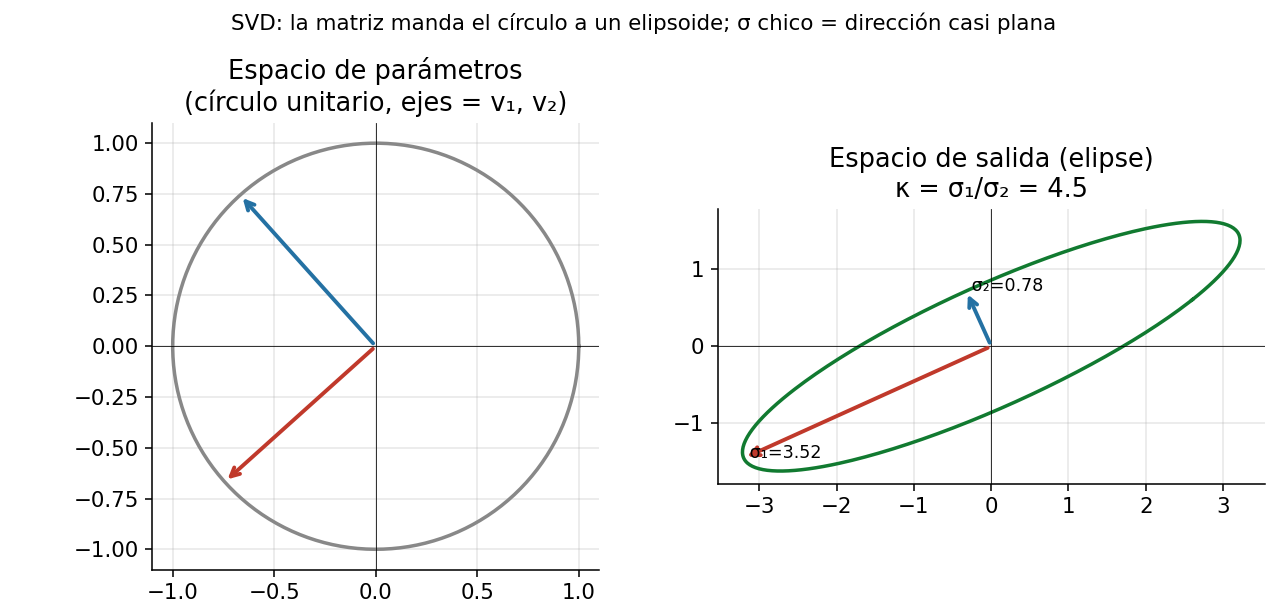
\includegraphics[width=0.72\linewidth]{fig_elipse_svd.png}
  \caption{Geometría de la SVD: la matriz $\J$ manda el círculo unitario del espacio de parámetros a un elipsoide en el espacio de observaciones. Los semiejes son los valores singulares $\sigma_k$ y sus orientaciones los vectores $\mathbf{u}_k$; el número de condición $\kappa=\sigma_{\max}/\sigma_{\min}$ mide cuán elongado (mal condicionado) es.}
  \label{fig:elipse}
\end{figure}

\paragraph{Número de condición.} La razón entre el eje mayor y el menor,
\begin{equation}
  \kappa(\J)=\frac{\sigma_{\max}}{\sigma_{\min}},
  \label{eq:kappa}
\end{equation}
resume en un número cuán elongado es el elipsoide. $\kappa\approx 1$ es una bola (todas las direcciones igual de determinadas); $\kappa$ grande significa que hay direcciones \emph{muchísimo} peor determinadas que otras --- problema mal condicionado. En WC, la SVD de $\tilde\J$ da $\kappa\approx 1.2\times 10^3$ (moderadamente mal condicionado) y señala que el valor singular más chico, $\sigma_{10}$, está \textbf{dominado por $w_{II}$}, con acoples débiles $a_e\!-\!\tau_e\!-\!w_{EE}$ y $a_i\!-\!\tau_i\!-\!\theta_i$. Este diagnóstico es puramente geométrico: no se entrenó ningún modelo todavía.

% ==========================================================================
\section{Matriz de información de Fisher (FIM)}
\label{sec:fisher}

\subsection*{Definición y forma operativa}
Supongamos ruido de observación gaussiano i.i.d.\ de varianza $\sigma_\varepsilon^2$: $\;\mathbf{y}=\mathbf{g}(\thetavec)+\bm{\varepsilon}$, $\bm{\varepsilon}\sim\mathcal{N}(0,\sigma_\varepsilon^2\mathbf{I})$. La \emph{matriz de información de Fisher} cuantifica cuánta información traen los datos sobre $\thetavec$ \cite{fisher1922}. Su definición es el valor esperado del producto exterior del gradiente de la log-verosimilitud $\log L$, y para este modelo se reduce a algo muy simple:
\begin{equation}
  \FIM(\thetavec)\;=\;\mathbb{E}\!\left[\Big(\tfrac{\partial \log L}{\partial\thetavec}\Big)\Big(\tfrac{\partial \log L}{\partial\thetavec}\Big)\transp\right]
  \;=\;\frac{1}{\sigma_\varepsilon^2}\,\J\transp\J .
  \label{eq:fim}
\end{equation}
La segunda igualdad es la clave operativa: \textbf{para ruido gaussiano, la FIM es (salvo el factor $1/\sigma_\varepsilon^2$) el producto $\J\transp\J$}. No hace falta calcular esperanzas: basta el Jacobiano de sensibilidad que ya teníamos.

\subsection*{Por qué la FIM ``es la curvatura del error''}
La log-verosimilitud es $\log L(\thetavec)=-\frac{1}{2\sigma_\varepsilon^2}\lVert\mathbf{y}-\mathbf{g}(\thetavec)\rVert^2+\text{cte}$, así que \emph{maximizar} la verosimilitud es \emph{minimizar} la superficie de error $L(\thetavec)=\frac{1}{2\sigma_\varepsilon^2}\lVert\mathbf{y}-\mathbf{g}(\thetavec)\rVert^2$ sobre el espacio de parámetros. Cerca del óptimo $\hat\thetavec$ el gradiente se anula, así que el desarrollo de Taylor a segundo orden deja solo el término cuadrático:
\begin{equation}
  L(\thetavec)\;\approx\; L(\hat\thetavec)+\tfrac12\,(\thetavec-\hat\thetavec)\transp \mathbf{H}\,(\thetavec-\hat\thetavec),
  \qquad \mathbf{H}=\text{Hessiano}\approx\FIM .
  \label{eq:taylor}
\end{equation}
Es decir: \textbf{la FIM es la matriz de curvatura del paisaje de error alrededor del óptimo}, un paraboloide cuya forma la fija $\FIM$. La lectura es directa:
\begin{itemize}[nosep]
  \item dirección \textbf{muy curvada} (autovalor grande) $\Rightarrow$ el error sube rápido al alejarse $\Rightarrow$ combinación \emph{bien determinada}, pico agudo de verosimilitud;
  \item dirección \textbf{plana} (autovalor chico) $\Rightarrow$ uno se mueve mucho sin que suba el error $\Rightarrow$ \emph{no identificable}, el ``valle plano''.
\end{itemize}

\subsection*{Fisher + SVD son una sola herramienta}
Sustituyendo la SVD \eqref{eq:svd} en \eqref{eq:fim} y usando que $\mathbf{U}\transp\mathbf{U}=\mathbf{I}$:
\begin{equation}
  \FIM=\frac{1}{\sigma_\varepsilon^2}\,\mathbf{V}\,\bm{\Sigma}^2\,\mathbf{V}\transp
  \quad\Longrightarrow\quad
  \underbrace{\lambda_k(\FIM)}_{\text{autovalor}}=\frac{\sigma_k^2}{\sigma_\varepsilon^2},
  \qquad \text{autovectores}=\mathbf{v}_k .
  \label{eq:fim-eig}
\end{equation}
O sea: \textbf{los autovectores de la FIM son exactamente las direcciones $\mathbf{v}_k$ de la SVD}, y sus autovalores son los $\sigma_k^2$ escalados por el ruido. Los ejes propios del paraboloide de error son las combinaciones $\mathbf{v}_k$; su curvatura es $\sigma_k^2/\sigma_\varepsilon^2$. Una dirección plana ($\sigma_k$ chico) es, a la vez, una dirección de poca curvatura y de poca información. Por eso ``analizar la FIM'' y ``hacer la SVD de $\J$'' son la misma operación, y todo el diagnóstico se puede hacer con una sola factorización. El método está tomado de Plate et al.\ para UDEs \cite{plate2024}.

\begin{figure}[H]
  \centering
  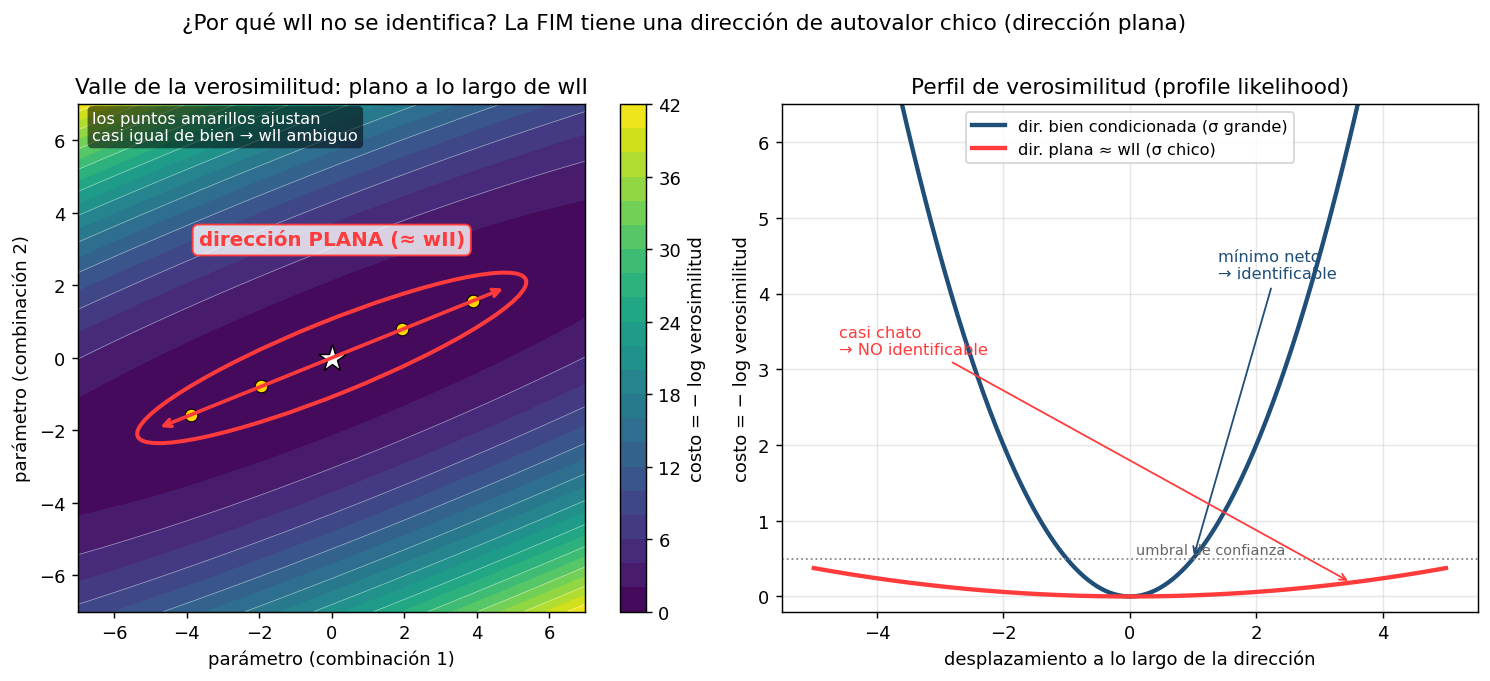
\includegraphics[width=0.80\linewidth]{valle_plano_svd_fim.png}
  \caption{El ``valle plano'' de la FIM en WC (figura del proyecto). El paisaje de error tiene una dirección muy curvada (bien identificable) y una casi plana; el eje del valle es la combinación $\mathbf{v}_{10}$, dominada por $w_{II}$. Moverse a lo largo del valle casi no cambia el error: esa es la firma geométrica de la no identificabilidad práctica.}
  \label{fig:valle}
\end{figure}

\begin{remark}[Valor singular vs.\ autovalor --- no confundir de quién es cada cosa]
$\J$ es \emph{rectangular} ($N\times p$): tiene \textbf{valores singulares} $\sigma_k$ (una matriz rectangular no tiene autovalores). La FIM $=\J\transp\J/\sigma_\varepsilon^2$ es \emph{cuadrada y simétrica} ($p\times p$): tiene \textbf{autovalores} $\lambda_k$. La relación es $\lambda_k(\FIM)=\sigma_k^2/\sigma_\varepsilon^2$: el autovalor de la FIM es el valor singular de $\J$ \emph{al cuadrado}, dividido por la varianza del ruido. Misma información, elevada al cuadrado y escalada. Cuidado también con la notación: $\sigma_k$ es un \emph{valor singular}, mientras que $\sigma_\varepsilon$ es el \emph{desvío del ruido}; son objetos distintos que comparten letra.
\end{remark}

% ==========================================================================
\section{Cota de Cramér--Rao: la incertidumbre correcta}
\label{sec:crb}

¿Cuál es el \emph{mejor} error posible al estimar $\thetavec$, aun con el estimador ideal? La \emph{cota de Cramér--Rao} (CRB) acota por debajo la covarianza de cualquier estimador insesgado \cite{rao1945,cramer1946}:
\begin{equation}
  \mathrm{Cov}(\hat{\thetavec}) \;\succeq\; \FIM^{-1}
  \;=\;\sigma_\varepsilon^2\,(\J\transp\J)^{-1}.
  \label{eq:crb}
\end{equation}
(El símbolo $\succeq$ significa que la diferencia $\mathrm{Cov}(\hat\thetavec)-\FIM^{-1}$ es semidefinida positiva.) La \textbf{desviación estándar mínima} del parámetro $j$ es la raíz del elemento diagonal de la \emph{inversa}:
\begin{equation}
  \mathrm{std}(\hat\theta_j)\;\ge\;\sigma_\varepsilon\,\sqrt{\big[(\J\transp\J)^{-1}\big]_{jj}}.
  \label{eq:crb-marginal}
\end{equation}
La conexión con la SVD es transparente: invertir la FIM es invertir $\bm{\Sigma}^2$, así que las direcciones planas ($\sigma_k$ chico) se transforman en \textbf{varianza enorme}. Curvatura chica $\to$ incertidumbre grande. El valle plano de la Figura~\ref{fig:valle} se paga como incertidumbre gigante en $w_{II}$.

\begin{remark}[Por qué la diagonal de la INVERSA, y no la norma de la columna]
Es el punto conceptual más importante del documento. Hay dos medidas que se confunden con facilidad:
\begin{itemize}[nosep]
  \item $\FIM_{jj}$, o equivalentemente $\lVert\J_{\cdot j}\rVert^2$: la sensibilidad \emph{marginal} ``bruta'' de $\theta_j$. \textbf{Ignora las correlaciones.}
  \item $(\FIM^{-1})_{jj}$: la incertidumbre \emph{real} de $\hat\theta_j$ teniendo en cuenta que se estima \emph{junto con todos los demás}.
\end{itemize}
Si $\theta_j$ está muy correlacionado con otro parámetro, $(\FIM^{-1})_{jj}$ se dispara aunque su columna $\lVert\J_{\cdot j}\rVert$ sea grande: puede tener mucha señal, pero señal \emph{redundante}, imposible de separar de la del vecino. Solo la inversa descuenta las correlaciones.
\end{remark}

\paragraph{El ejemplo del proyecto: ``box'' vs.\ ``chirp''.} Este error tuvo consecuencias concretas al elegir el estímulo para identificar $w_{II}$ (experimento C). La métrica ingenua $\lVert$columna$\rVert$ decía que el pulso cuadrado (``box'') era el mejor estímulo, porque produce una señal de amplitud grande. Pero la CRB correcta $\sqrt{\mathrm{diag}(\FIM^{-1})}$ dice lo contrario: el mejor es el \textbf{chirp} (barrido de frecuencia). ¿Por qué? El box excita $E$ e $I$ casi en fase ($E\approx I$), de modo que sus sensibilidades quedan \emph{correlacionadas} --- señal grande pero redundante. El chirp, de banda ancha, \emph{decorrelaciona} las direcciones y por eso baja la CRB de $w_{II}$. Moraleja: identificabilidad $=$ sensibilidad \emph{decorrelacionada}, no amplitud.

% ==========================================================================
\section{Identificabilidad estructural vs.\ práctica}
\label{sec:identif}

Conviene separar dos preguntas que suenan parecido pero no lo son:
\begin{itemize}[nosep]
  \item \textbf{Identificabilidad estructural.} En el mundo ideal --- datos infinitos y \emph{sin ruido} --- ¿existe un único $\thetavec$ que produce esa salida? Es una propiedad de la \emph{estructura} del modelo. Por ejemplo, dos parámetros que solo aparecen como producto $w_1 w_2$ nunca se separan: son estructuralmente no identificables.
  \item \textbf{Identificabilidad práctica.} Con \emph{ruido finito y datos finitos}, ¿está el parámetro bien determinado? Un parámetro puede ser estructuralmente identificable y aun así vivir en una dirección casi plana, con lo cual el ruido lo vuelve \emph{prácticamente} no identificable. Es lo que miden la FIM y la CRB.
\end{itemize}

\paragraph{El caso de $w_{II}$.} En WC, $w_{II}$ es \textbf{estructuralmente identificable} --- se lo recupera bien usando múltiples trayectorias con datos limpios --- pero \textbf{prácticamente mal identificable bajo ruido}: su CRB es alta y, como veremos en \S\ref{sec:hallazgo}, su recuperación se degrada dramáticamente cuando sube $\sigma_\varepsilon$. La distinción es fundamental porque los remedios difieren: contra la no identificabilidad estructural hay que \emph{cambiar el modelo o la parametrización}; contra la práctica alcanza con \emph{más/mejores datos} (OED), \emph{fijar} o \emph{regularizar}.

\paragraph{Profile likelihood.} El método canónico para diagnosticar identificabilidad práctica es el \emph{profile likelihood} de Raue et al.\ \cite{raue2009}: se fija $\theta_j$ en un rango de valores, se reoptimiza \emph{todo el resto} en cada valor y se traza la verosimilitud resultante. Un perfil con un \textbf{valle marcado} en torno a $\hat\theta_j$ indica que el dato ``castiga'' alejarse $\Rightarrow$ identificable. Un perfil \textbf{plano} indica que se puede mover $\theta_j$ sin empeorar el ajuste (reacomodando los demás) $\Rightarrow$ no identificable. Es la versión \emph{global y no lineal} de mirar el autovalor chico de la FIM: la FIM es la aproximación local cuadrática \eqref{eq:taylor}, y el profile likelihood explora el valle completo, incluso lejos del óptimo.

% ==========================================================================
\section{Remedios: qué fijar, cómo regularizar, qué estímulo usar}
\label{sec:remedios}

Diagnosticado el problema (\S\ref{sec:svd}--\ref{sec:identif}), hay tres familias de remedios, que en el proyecto corresponden a los experimentos B, A y C. La idea unificadora es que los tres \emph{agregan información} a las direcciones planas de la FIM.

\subsection{Selección de subconjuntos por QR con pivoteo (Exp.\ B)}
\label{sec:subset}
Si liberar los 10 parámetros es mal condicionado, una estrategia establecida es \textbf{fijar} los peor identificables en un valor previo/nominal y estimar solo el subconjunto bien condicionado \cite{chu2007}. ¿Cuáles fijar? La respuesta la da la geometría de $\J$.

\paragraph{QR con pivoteo de columnas.} Se aplica la factorización $\tilde\J\,\bm{\Pi}=\mathbf{Q}\mathbf{R}$, donde $\bm{\Pi}$ es una permutación que \emph{reordena} las columnas (parámetros) de mayor a menor independencia lineal (pivotes $|R_{ii}|$ decrecientes) \cite{golub2013}. La \emph{cola} del ranking --- los últimos pivotes --- son los parámetros que más ``se explican'' con combinaciones de los demás: los candidatos naturales a fijar. Es una selección \emph{greedy} por ortogonalización, equivalente a mirar los $\mathbf{v}_k$ de los $\sigma_k$ chicos (\S\ref{sec:svd}) y fijar un representante de cada dirección débil. En WC, el QR-pivoteo dio el orden $\theta_e>\dots>a_e>w_{II}$, con $w_{II}$ en último lugar y cola $\{w_{EI},a_e,w_{II}\}$.

\begin{remark}[Regla práctica: fijar de más empeora]
Fijar un \emph{representante mínimo} de cada acople débil ayuda; fijar \emph{de más} sobre-restringe y \emph{empeora}. En WC, fijar $w_{II}$ \emph{o} $a_i$ (ambos viven en la ecuación de la población inhibitoria) baja mucho el error del resto. Pero fijar \emph{los dos a la vez} rompe el acople $a_i\!\leftrightarrow\!w_{II}$ y dispara el error: el subconjunto queda sobre-restringido. La regla es fijar uno por acople débil, no todos.
\end{remark}

\subsection{Regularización de Tikhonov / ridge / MAP (Exp.\ A)}
\label{sec:reg}
En lugar de fijar un parámetro de golpe, se puede \textbf{penalizar} su alejamiento de un valor previo $\thetavec^0$ (regularización de Tikhonov / ridge) \cite{tikhonov1977}:
\begin{equation}
  \hat{\thetavec}=\arg\min_{\thetavec}\;\underbrace{\lVert \mathbf{y}-\mathbf{g}(\thetavec)\rVert^2}_{\text{ajuste}}
  \;+\;\lambda\underbrace{\lVert \thetavec-\thetavec^{0}\rVert^2}_{\text{penalización}} .
  \label{eq:ridge}
\end{equation}
Tres lecturas equivalentes del mismo objeto:
\begin{itemize}[nosep]
  \item \textbf{Ridge / Tikhonov:} sumar $\lambda\mathbf{I}$ a la FIM ($\FIM+\lambda\mathbf{I}$) le agrega curvatura a las direcciones planas y la vuelve invertible / mejor condicionada.
  \item \textbf{MAP bayesiano:} \eqref{eq:ridge} es el máximo a posteriori con un \emph{prior} gaussiano $\thetavec\sim\mathcal{N}(\thetavec^0,\tau^2\mathbf{I})$, con $\lambda=\sigma_\varepsilon^2/\tau^2$. El prior aporta la información que faltaba en el valle.
  \item \textbf{Sesgo--varianza:} se agrega \emph{sesgo} (hacia $\thetavec^0$) a cambio de \emph{menos varianza}, y eso conviene justo en las direcciones mal condicionadas.
\end{itemize}

\begin{remark}[El continuo $\lambda\to\infty\equiv$ fijar]
Con $\lambda=0$ se recupera el ajuste libre (10 parámetros sueltos); con $\lambda\to\infty$ el parámetro queda clavado en $\theta_j^0$, es decir, equivale a \emph{fijarlo} (\S\ref{sec:subset}). La regularización es entonces el \emph{continuo} entre ``todo libre'' y ``fijar'', y un $\lambda$ intermedio suele ser óptimo.
\end{remark}

\begin{figure}[H]
  \centering
  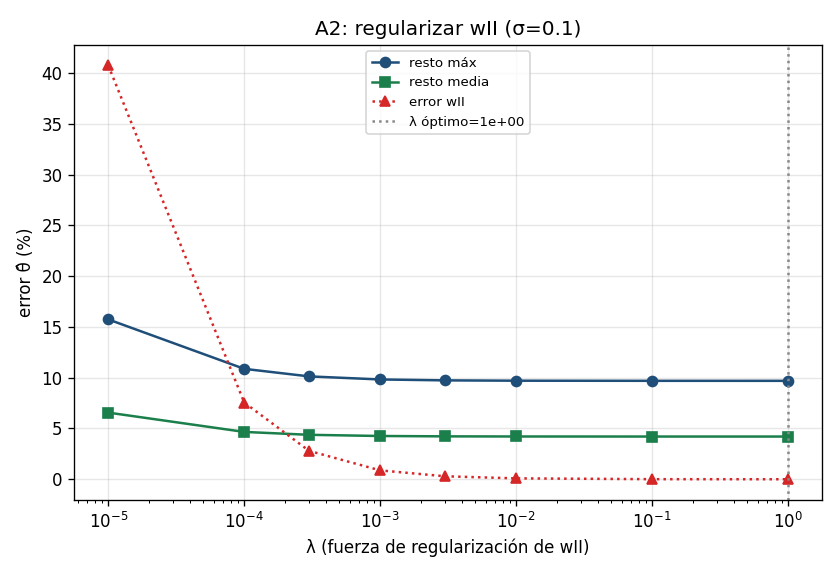
\includegraphics[width=0.80\linewidth]{expA2_reg_lambda.png}
  \caption{Barrido del parámetro de regularización $\lambda$ sobre $w_{II}$ (figura del proyecto). El error de los demás parámetros baja de forma monótona con $\lambda$ y \emph{satura} en el valor que se obtiene al fijar $w_{II}$: es la confirmación empírica de que $\lambda\to\infty$ equivale a fijar. El óptimo práctico está en $\lambda\approx 1$.}
  \label{fig:reglambda}
\end{figure}

\subsection{Diseño óptimo de experimentos (OED) --- el estímulo ES la información (Exp.\ C)}
\label{sec:oed}
La FIM depende de la trayectoria, y la trayectoria depende del \emph{estímulo} $P(t),Q(t)$. Luego \textbf{elegir el estímulo es elegir la información}: es el diseño óptimo de experimentos (OED) o diseño de entrada óptimo \cite{ljung1999,franceschini2008,plate2024}. A diferencia de fijar o regularizar --- que reparten mejor información escasa --- el OED \emph{crea} información nueva. Se optimiza un funcional escalar de la FIM:
\begin{center}
\begin{tabular}{ll}
  \toprule
  \textbf{A-óptimo} & minimizar $\mathrm{tr}(\FIM^{-1})$ --- varianza media de los estimadores (suma de CRB$^2$)\\
  \textbf{D-óptimo} & maximizar $\det(\FIM)$ --- mínimo volumen del elipsoide de confianza\\
  \textbf{E-óptimo} & maximizar $\lambda_{\min}(\FIM)$ --- mejora la \emph{peor} dirección (la más débil)\\
  \bottomrule
\end{tabular}
\end{center}

\paragraph{Excitación persistente (Ljung).} Para identificar un sistema hay que \emph{recorrer} su espacio de estados: una entrada demasiado pobre (casi constante) deja direcciones sin excitar y la FIM sin rango completo. Una entrada es \emph{persistentemente excitante} si su contenido espectral cubre las dinámicas del sistema \cite{ljung1999}. Por eso los estímulos de banda ancha (chirp, secuencias pseudoaleatorias PRBS, Poisson) condicionan mucho mejor la FIM que un pulso cuadrado, aunque este tenga más amplitud (Figura~\ref{fig:oedcond}): lo que importa no es la energía, sino la \emph{decorrelación} de las direcciones sensibles. En WC, además, todos los estímulos deben ser \emph{realizables con optogenética} (on/off, $\geq 0$), lo que restringe el diseño a señales no negativas.

\begin{figure}[H]
  \centering
  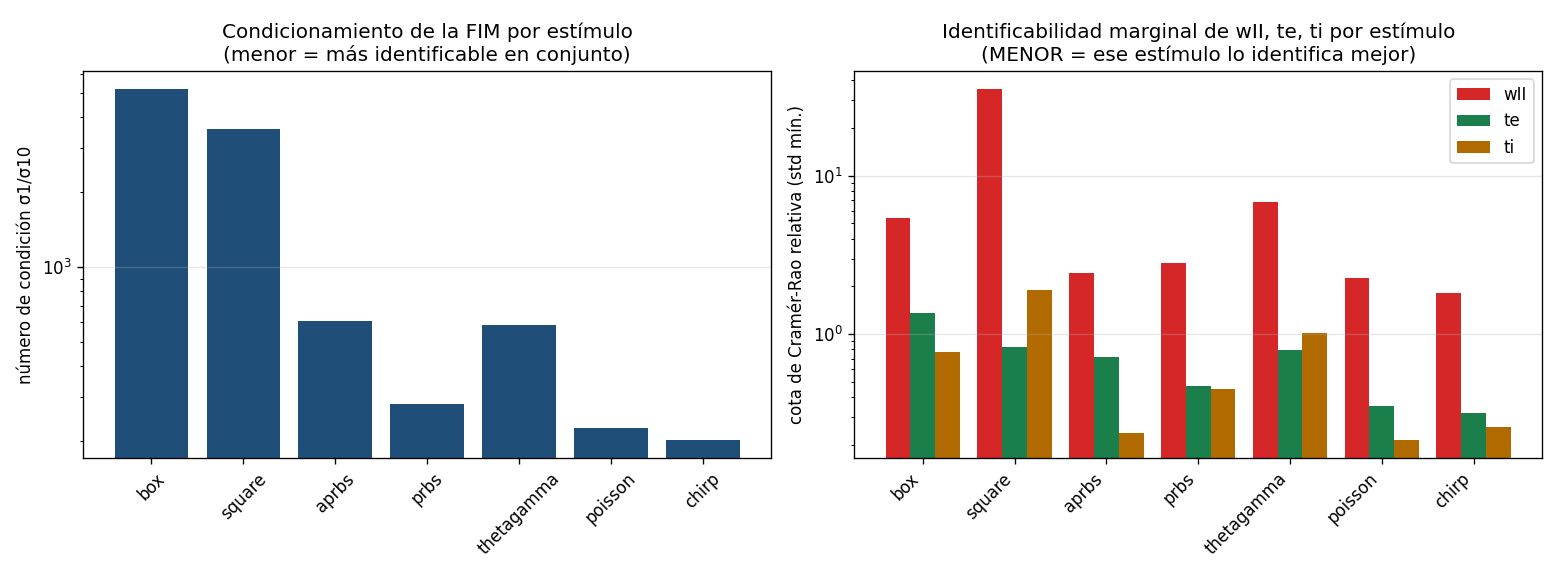
\includegraphics[width=0.80\linewidth]{oed_cond_por_estimulo.png}
  \caption{Número de condición $\kappa$ de la FIM por familia de estímulo (figura del proyecto). Los estímulos de banda ancha (chirp, Poisson, PRBS) dan $\kappa$ mucho menor --- FIM mejor condicionada --- que el box/square, pese a que estos últimos tienen mayor amplitud. La banda ancha decorrelaciona las direcciones sensibles.}
  \label{fig:oedcond}
\end{figure}

\paragraph{OED ponderado al cuello de botella.} A ruido moderado, una \emph{mezcla} de estímulos complementarios maximiza la identificabilidad conjunta. Pero a ruido extremo, el cuello de botella ($w_{II}$) necesita \emph{peso extra} en su dirección propia (típicamente más excitación por $Q$, la entrada a la población inhibitoria). El OED ponderado --- que sacrifica un poco de información global para volcarla en la dirección débil --- muestra un óptimo interior (Figura~\ref{fig:oedweighted}): ni cobertura uniforme ni todo al cuello de botella, sino un punto medio. Es el mismo compromiso sesgo--varianza de la regularización, ahora en el diseño del experimento.

\begin{figure}[H]
  \centering
  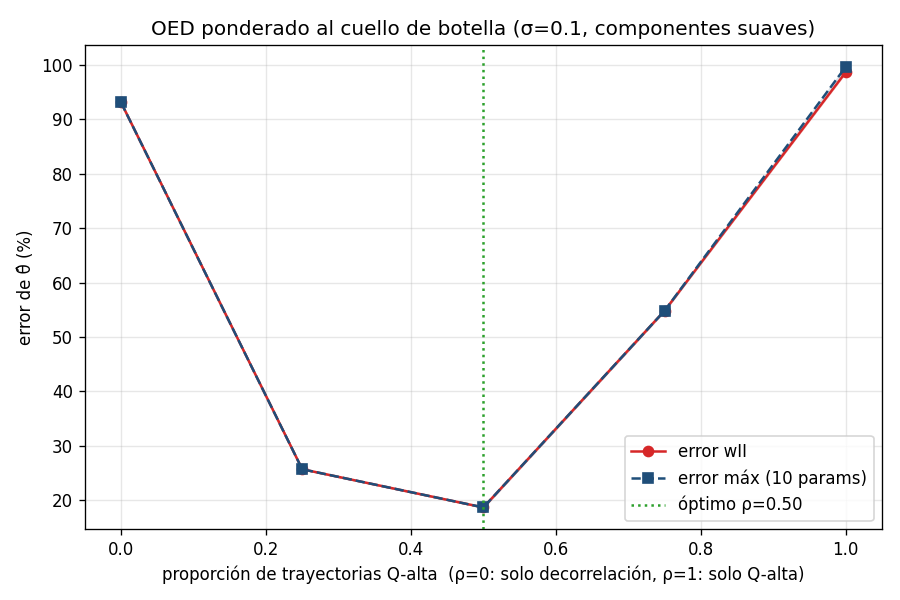
\includegraphics[width=0.72\linewidth]{oed_weighted.png}
  \caption{OED ponderado (figura del proyecto): error de identificación en función del peso $\rho$ dado a la dirección del cuello de botella. La curva tiene forma de V con óptimo interior en $\rho\approx 0.5$: repartir toda la información de manera uniforme ($\rho\to 0$) o volcarla entera al cuello de botella ($\rho\to 1$) son ambos peores que el balance intermedio.}
  \label{fig:oedweighted}
\end{figure}

% ==========================================================================
\section{El hallazgo del proyecto: $w_{II}$ vive en la dirección plana}
\label{sec:hallazgo}

Todo el aparato anterior converge en un resultado limpio y verificable, que es el corazón de esta etapa del proyecto.

\paragraph{Predicho sin entrenar.} La SVD de la FIM (evaluada en $\thetavec^\star$, \emph{antes de ajustar ningún modelo}) señaló que el valor singular más chico está dominado por $w_{II}$: el parámetro vive en la dirección plana del valle (Figura~\ref{fig:valle}). Este es un diagnóstico puramente geométrico --- la FIM \emph{predice} el cuello de botella sin que se haya entrenado un solo Neural ODE. Es la promesa de la herramienta: saber de antemano qué se va a poder recuperar y qué no.

\paragraph{Confirmado bajo ruido.} El barrido de ruido (Figura~\ref{fig:noise}) confirma la predicción de manera contundente. Con datos limpios, $w_{II}$ se recupera con un error del $0.8\%$; al subir el ruido a $\sigma_\varepsilon=0.10$, su error se dispara al $41\%$, mientras que los parámetros que viven en direcciones curvadas se mantienen estables. La FIM había dicho ``$w_{II}$ es frágil'', y el experimento la confirmó. Predicción y verificación cierran el círculo diagnóstico.

\begin{figure}[H]
  \centering
  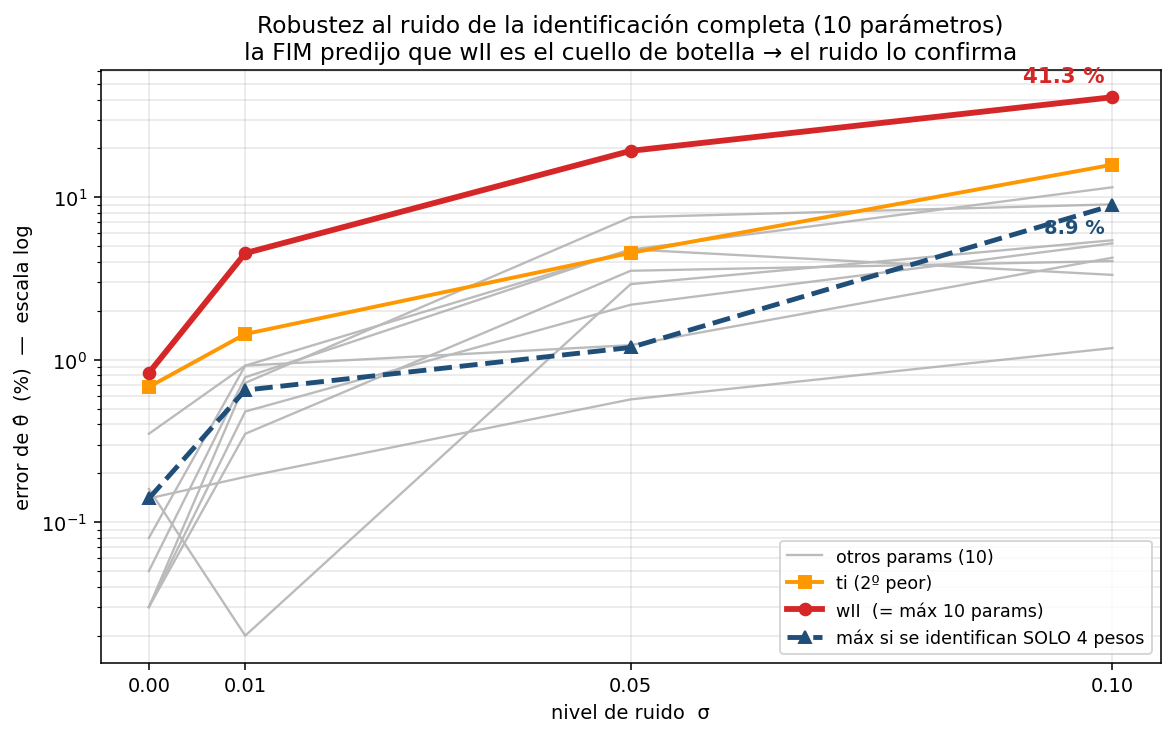
\includegraphics[width=0.82\linewidth]{noise_param_error.png}
  \caption{Error de identificación por parámetro en función del nivel de ruido $\sigma_\varepsilon$ (figura del proyecto). $w_{II}$ (el parámetro de la dirección plana) es de lejos el que peor escala: pasa de $\sim 0.8\%$ con datos limpios a $\sim 41\%$ a $\sigma_\varepsilon=0.10$. Los parámetros en direcciones curvadas apenas se degradan. La FIM había anticipado exactamente esta jerarquía.}
  \label{fig:noise}
\end{figure}

\paragraph{Pero la fragilidad no se propaga al control (adelanto de B5).} Sería fácil concluir que un $w_{II}$ mal identificado arruina cualquier uso posterior del modelo. \emph{No es así}, y este es un matiz importante. El objetivo último del proyecto no es estimar $\thetavec$ por sí mismo, sino usar el modelo identificado para \textbf{controlar} el sistema en lazo cerrado (un controlador IMC que lleva el régimen al objetivo theta-gamma). Resulta que la dirección plana en la que vive $w_{II}$ es, en buena medida, una dirección a la que el controlador es \emph{insensible}: el mismo mecanismo (colinealidad $E\approx I$) que hace a $w_{II}$ difícil de estimar también lo hace poco relevante para el comportamiento entrada--salida que el control necesita reproducir. Por eso la incertidumbre grande en $w_{II}$ \textbf{no se propaga} al desempeño de control. La lección es que ``identificabilidad'' debe leerse \emph{orientada a la tarea}: un parámetro puede ser prácticamente no identificable y, aun así, irrelevante para el objetivo final. El desarrollo cuantitativo de este punto está en B5 (validación orientada al control).

% ==========================================================================
\begin{thebibliography}{99}
\bibitem{golub2013} G.~H.~Golub y C.~F.~Van Loan, \emph{Matrix Computations}, 4.\textsuperscript{a} ed., Johns Hopkins University Press, 2013.
\bibitem{fisher1922} R.~A.~Fisher, ``On the mathematical foundations of theoretical statistics'', \emph{Phil.\ Trans.\ R.\ Soc.\ A}, 222:309--368, 1922.
\bibitem{rao1945} C.~R.~Rao, ``Information and the accuracy attainable in the estimation of statistical parameters'', \emph{Bull.\ Calcutta Math.\ Soc.}, 37:81--89, 1945.
\bibitem{cramer1946} H.~Cramér, \emph{Mathematical Methods of Statistics}, Princeton University Press, 1946.
\bibitem{raue2009} A.~Raue \emph{et al.}, ``Structural and practical identifiability analysis of partially observed dynamical models by exploiting the profile likelihood'', \emph{Bioinformatics}, 25(15):1923--1929, 2009.
\bibitem{chu2007} Y.~Chu y J.~Hahn, ``Parameter set selection for estimation of nonlinear dynamic systems'', \emph{AIChE Journal}, 53(11):2858--2870, 2007.
\bibitem{tikhonov1977} A.~N.~Tikhonov y V.~Y.~Arsenin, \emph{Solutions of Ill-Posed Problems}, Winston \& Sons, 1977.
\bibitem{ljung1999} L.~Ljung, \emph{System Identification: Theory for the User}, 2.\textsuperscript{a} ed., Prentice Hall, 1999.
\bibitem{franceschini2008} G.~Franceschini y S.~Macchietto, ``Model-based design of experiments for parameter precision: State of the art'', \emph{Chem.\ Eng.\ Sci.}, 63(19):4846--4872, 2008.
\bibitem{plate2024} C.~Plate \emph{et al.}, ``Optimal experimental design for universal differential equations'', 2024 (preprint arXiv).
\end{thebibliography}

\end{document}
